\section{Activity Diagrams}

\subsection{Self Registration}

The use case starts when a user accesses the register page (or clicks the register button on the login form), and then a register form will be displayed. The user provided some information (including email, password, and name). Then,  the provided information is verified. If it is valid, a confirmation email will be sent to the user. After accessing the link in the email, a new account is created and the user can log into the system.

\begin{figure}[H]
  \centering
  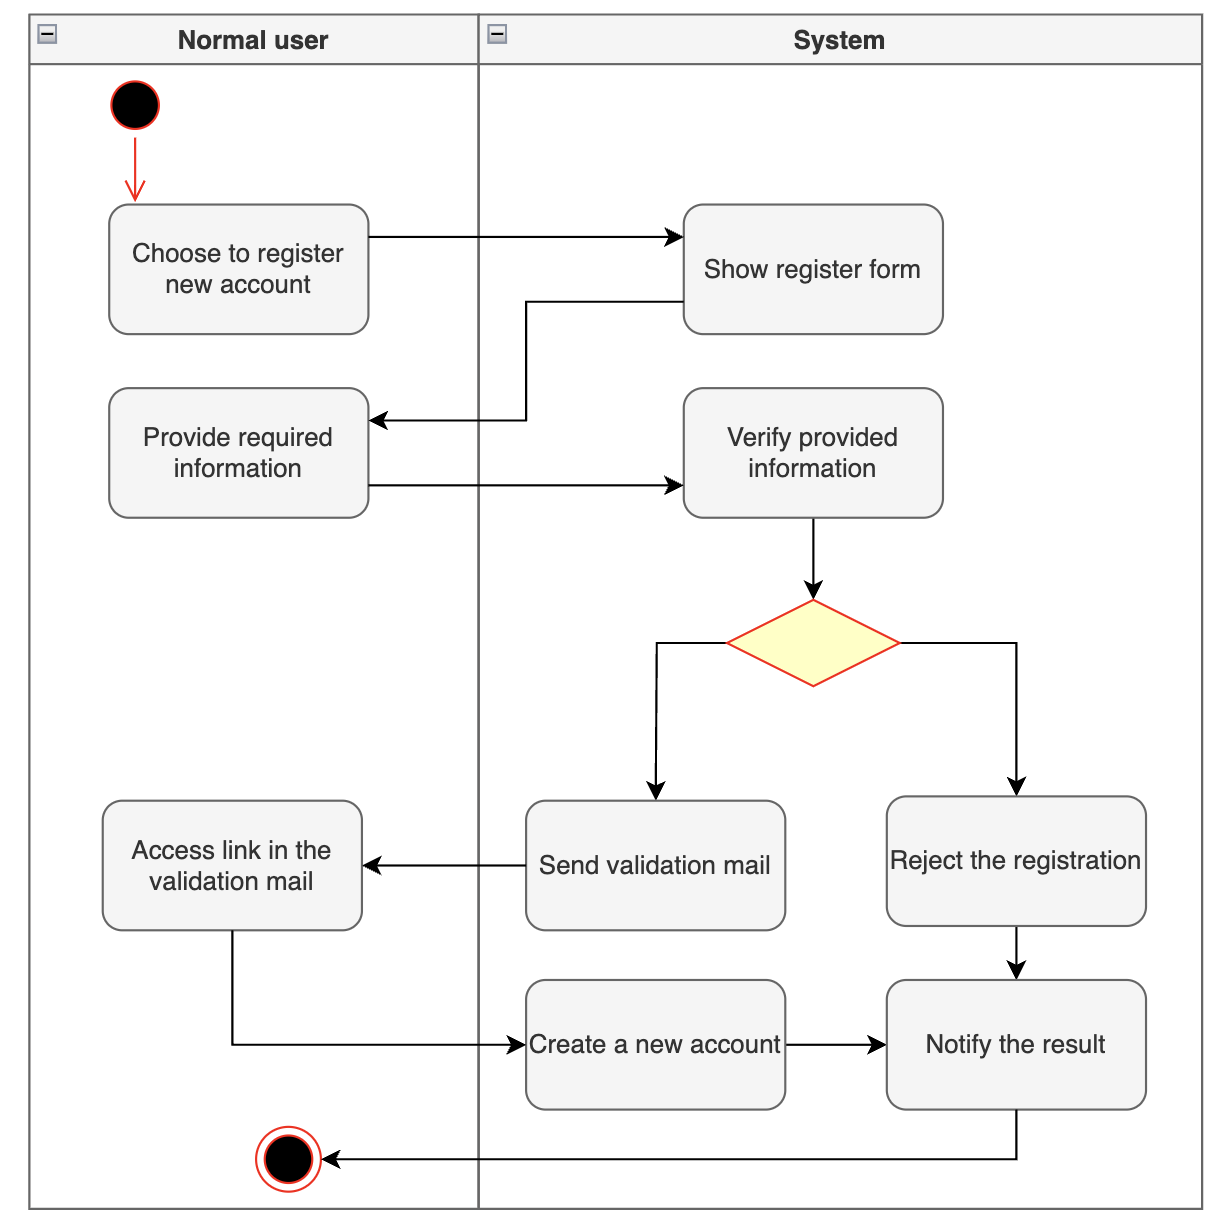
\includegraphics[width=0.7\textwidth]{Figures/self_register.png}
  \caption{Self Registration activity diagram}
  \label{fig:self-registration}
\end{figure}


\subsection{Login}

The use case starts when an unauthorized user tries to access internal features or goes to the login page. The user at the login can provide an email and password and send them to the system. If the credential information is valid, the user will be granted access permission and navigated to an internal page. Otherwise, an error alert will be displayed.

\begin{figure}[H]
  \centering
  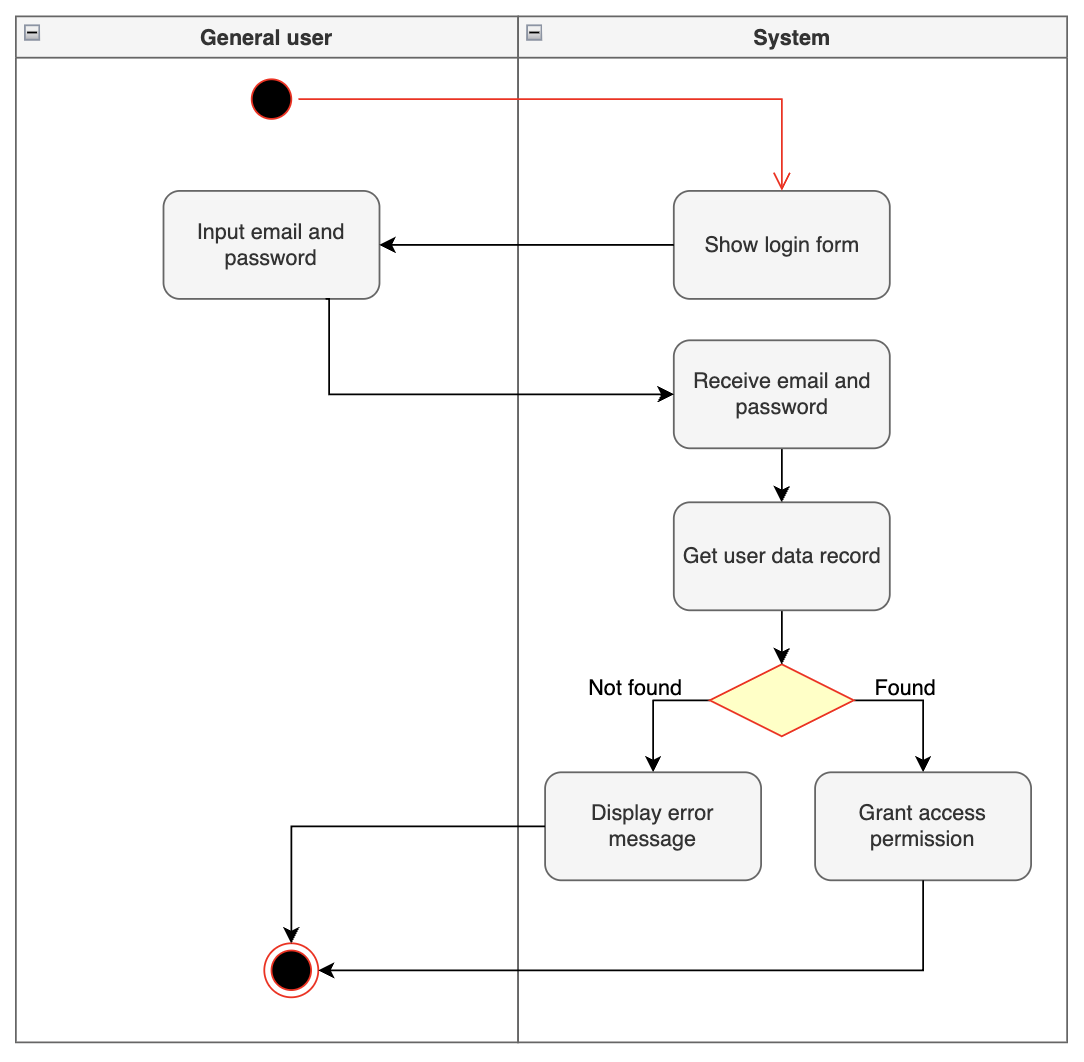
\includegraphics[width=0.7\textwidth]{Figures/login.png}
  \caption{Login activity diagram}
  \label{fig:login}
\end{figure}

\subsection{Login with a Google account}

The use case starts when a user chooses the option of logging in with a Google account, then a Google login form will be displayed. Users provide Google authentication information. Google Auth service verifies the authentication information and generates an access token. Finally, the system validates the access token and grants access permission to the user.

\begin{figure}[H]
  \centering
  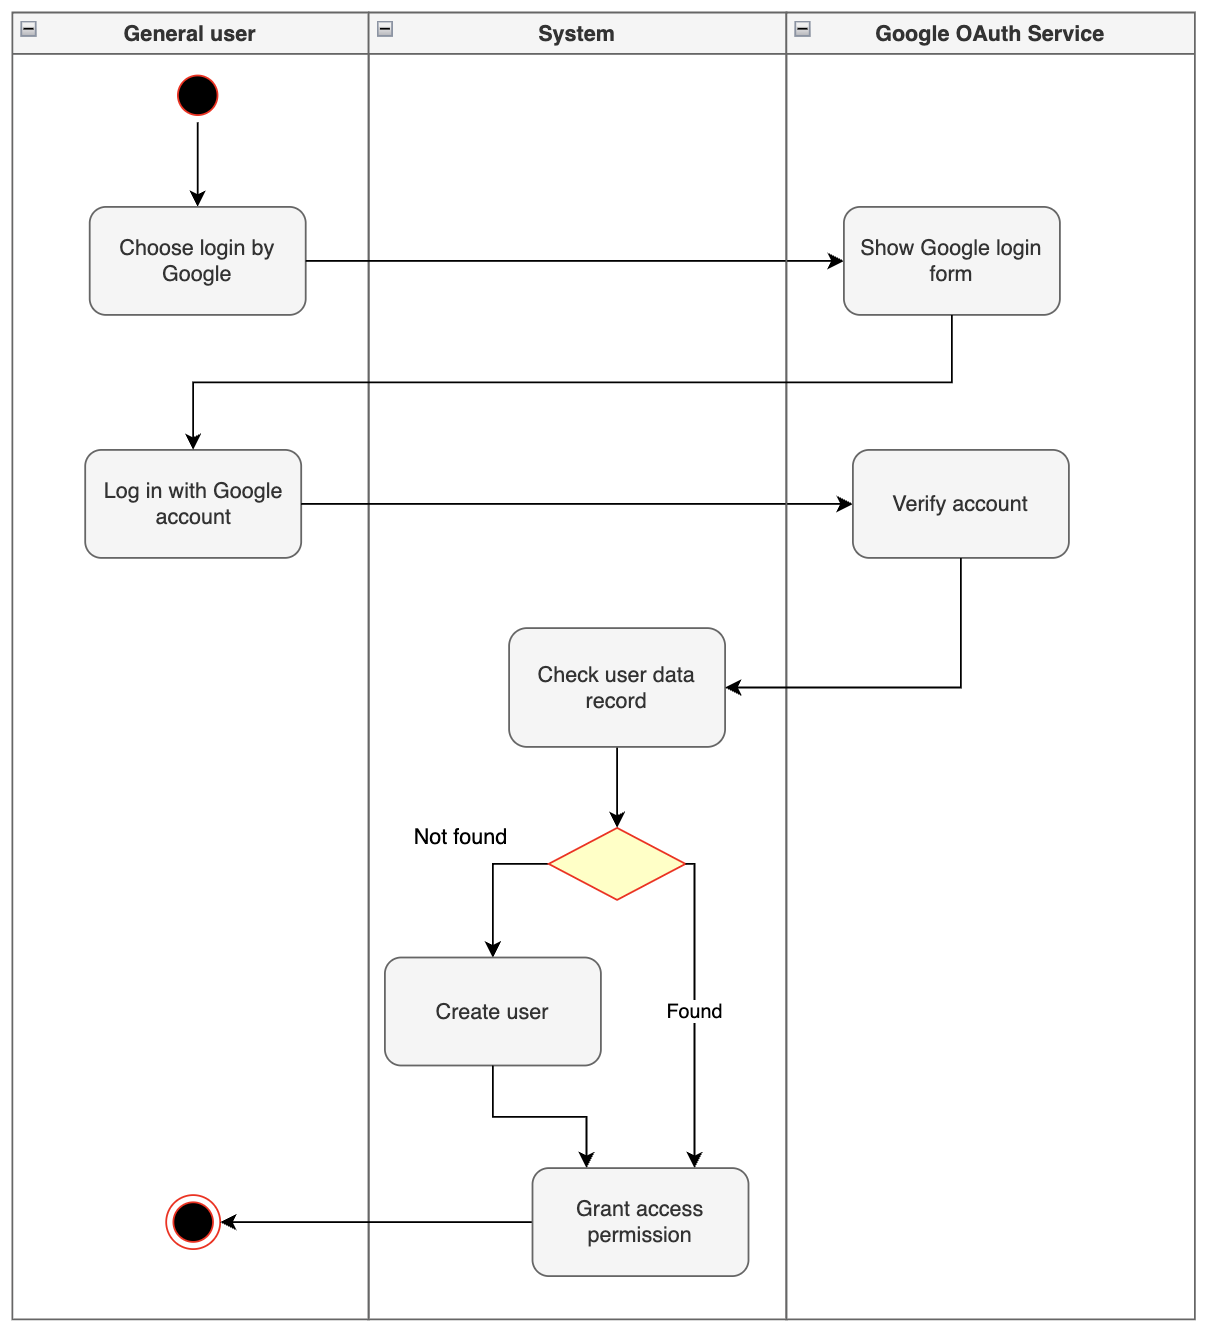
\includegraphics[width=0.7\textwidth]{Figures/login_gg.png}
  \caption{Login with a Google account activity diagram}
  \label{fig:login-google}
\end{figure}

\subsection{Update to Organization account}

The use case starts when an individual user chooses to update to organization accounts, then a form will be displayed. Then, users provide some information for verification and submit them. After the update-account application is verified by admins, the system updates the account and notifies the user of the results.

\begin{figure}[H]
  \centering
  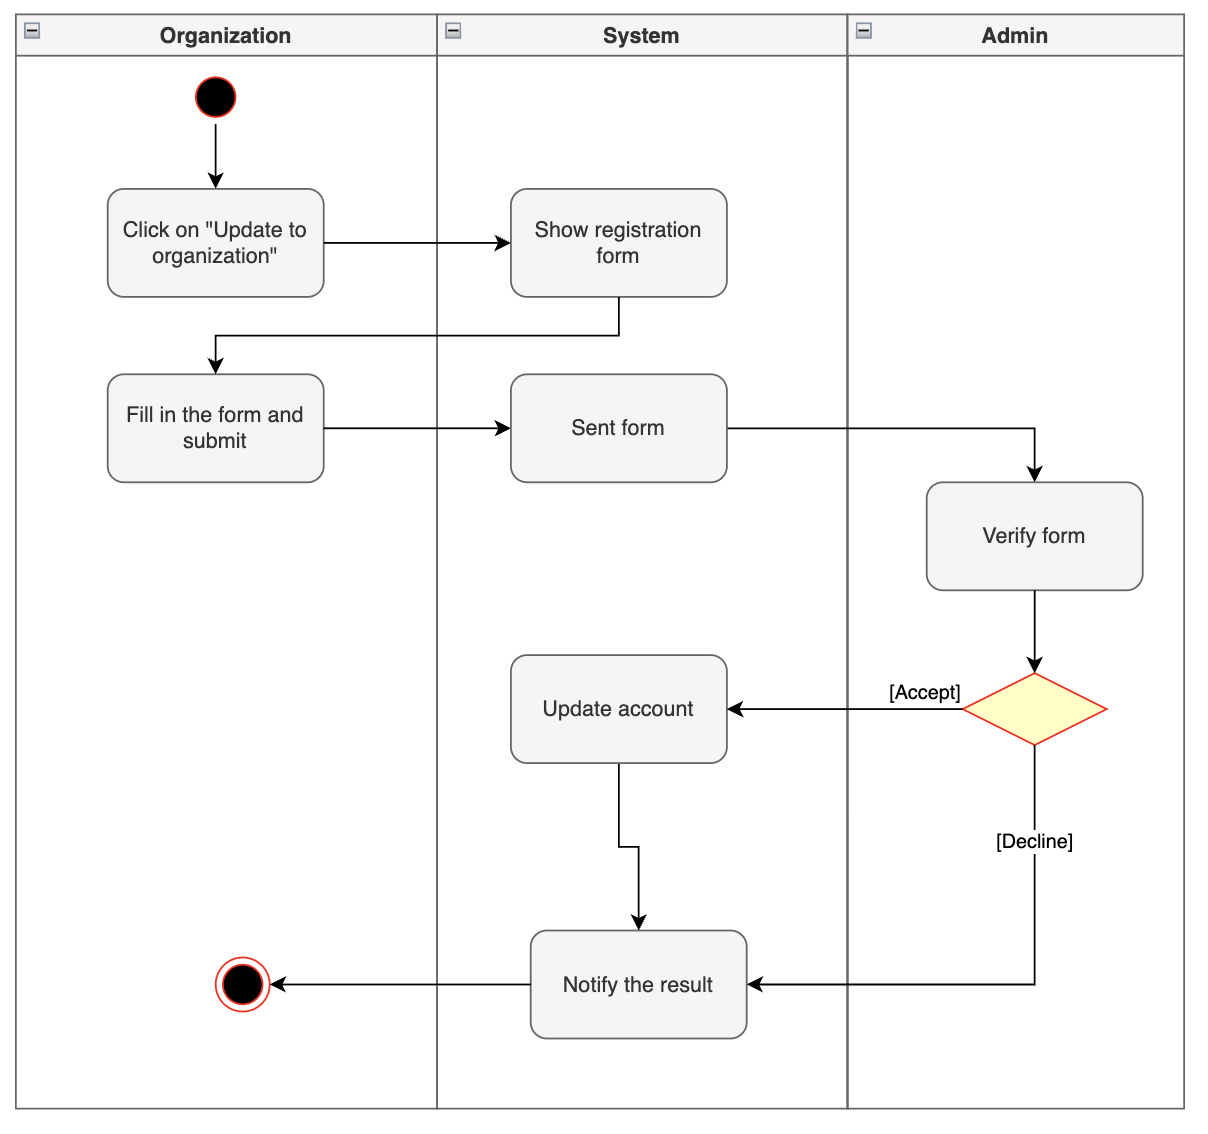
\includegraphics[width=0.7\textwidth]{Figures/update_org.png}
  \caption{Update to Organization account activity diagram}
  \label{fig:update-org}
\end{figure}

\subsection{Manage pet profiles}


\begin{figure}[H]
  \centering
  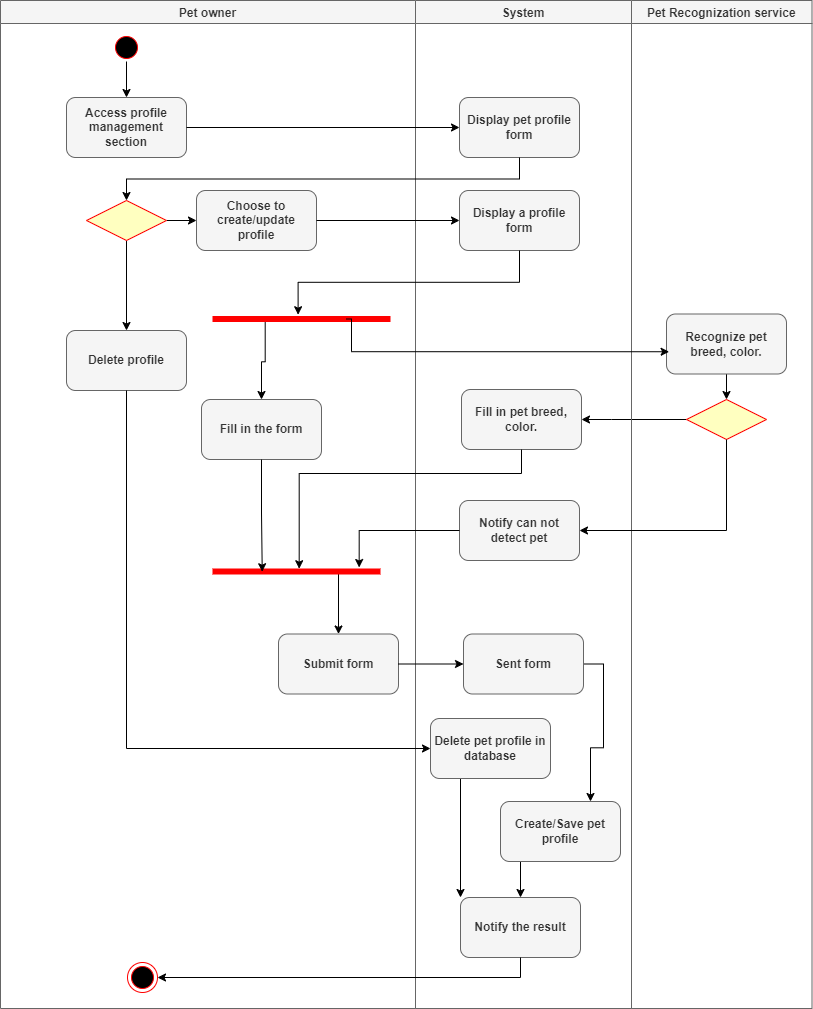
\includegraphics[width=0.7\textwidth]{Figures/manage_pet.png}
  \caption{Manage pet profile activity diagram}
  \label{fig:manage-pet}
\end{figure}

The use case starts when a user accesses the pet profile management page. The user chooses to edit or create a new profile and a form will be displayed. Note that the form would be filled if the user chose to edit an available profile. In that case, the user can modify the fields or rather delete the profile. Otherwise, the user can input the pet information and submit it. The user can also fill in pet breeds and colors by providing images. Finally, the content of the form will be verified, and the result will be displayed.


\subsection{Access pet profile}

In the pet profile page, a user has options to find pets by filtering by categories or providing pet images. In case the user filters by images, those images will be processed by the Pet Recognition Service. Then, the filtered pet profiles will be displayed to the user. The user can click on pet profiles for further information or continue finding other pet profiles.

\begin{figure}[H]
  \centering
  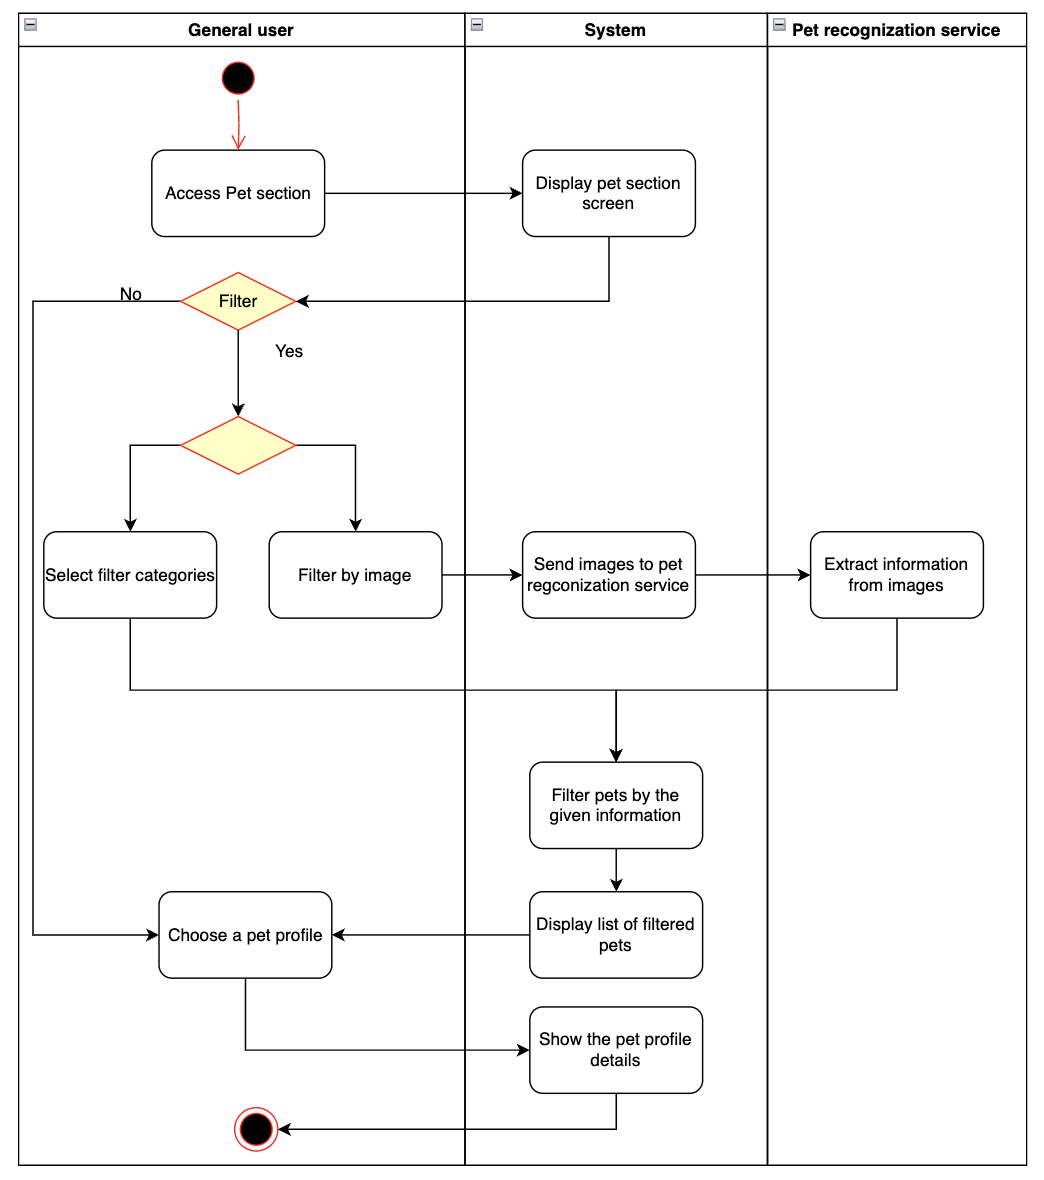
\includegraphics[width=0.7\textwidth]{Figures/access_pet.png}
  \caption{Access pet profile activity diagram}
  \label{fig:access-pet}
\end{figure}

\subsection{Adopt pets}

After finding a pet profile successfully, if the pet is still available, a user can choose to adopt the pet by filling in the required information in the adoption form and sending it. The application form will be reviewed by the pet owner. The result will be sent to the user then. Note that, the user can still contact directly to the pet owner during the pet adoption process.

\begin{figure}[H]
  \centering
  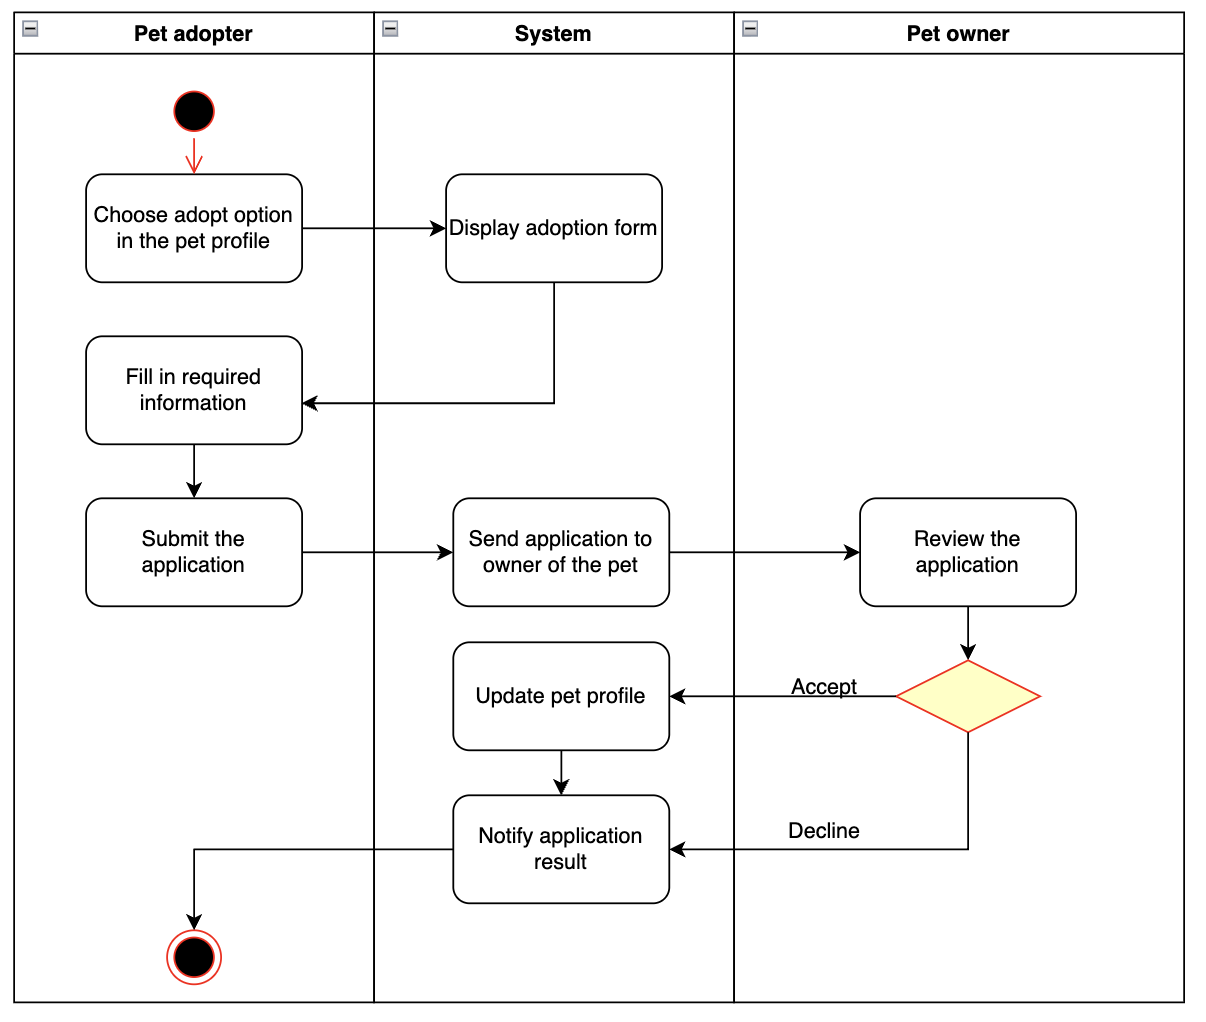
\includegraphics[width=0.7\textwidth]{Figures/adopt_pet.png}
  \caption{Adopt pets activity diagram}
  \label{fig:adopt-pet}
\end{figure}

\subsection{Interact with posts}

After accessing a pet profile successfully, a user can also see public posts of the pet. The user can choose a post for further information and leave their comments or likes on the post. Note that the private posts can only be seen by the pet owner and admins.

\begin{figure}[H]
  \centering
  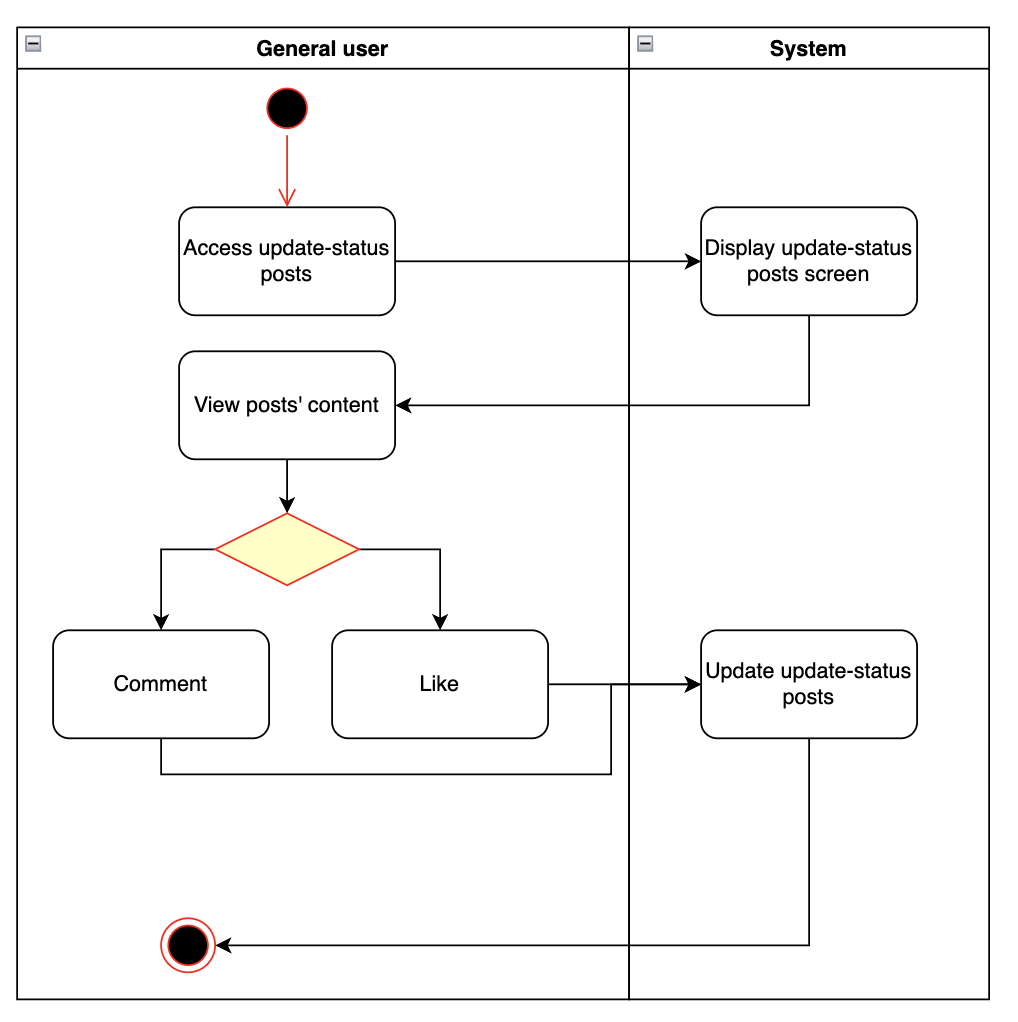
\includegraphics[width=0.7\textwidth]{Figures/post_interact.png}
  \caption{Interact with posts activity diagram}
  \label{fig:interact-post}
\end{figure}

\subsection*{Create posts}

\begin{figure}[H]
  \centering
  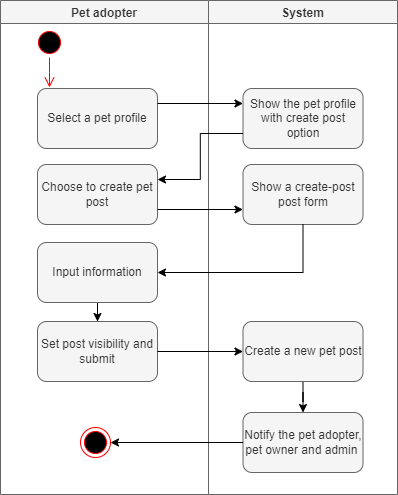
\includegraphics[width=0.7\textwidth]{Figures/create-pet-post.png}
  \caption{Create posts activity diagram}
  \label{fig:create-post}
\end{figure}

Updating the status of a pet is uploading posts about it. The use case starts when an owner can select a pet profile and choose the option of updating the pet status. After filling information, the owner can set visibility for the post. Finally, the user can send the form and a new post is created.


\subsection{Manage blogs}

The use case starts when a user with an Organization account accesses the blog management page. The user chooses to edit or create a new blog, then a form will be displayed. Note that the form would be filled if the user chose to edit an available blog. In that case, the user can modify the fields or rather delete the blog. If the user wants to create a new blog, the user can input and submit it. Finally, admins will verify the blog and the result will be sent to the user.

\begin {figure}[H]
\centering
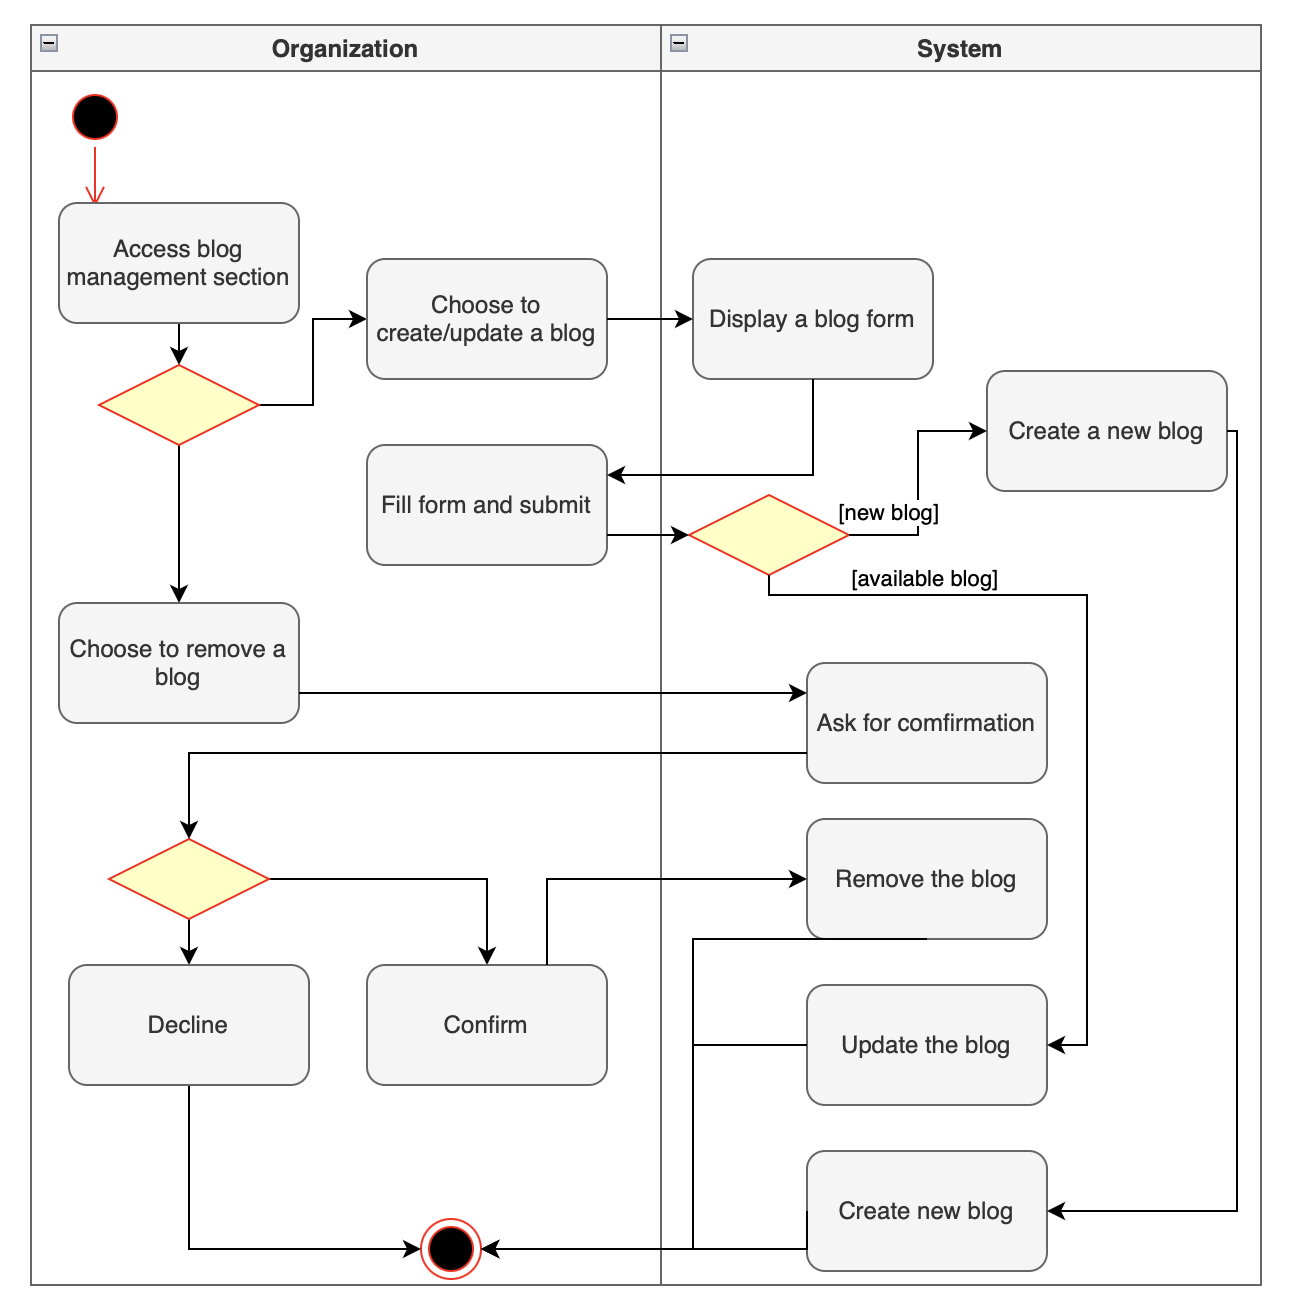
\includegraphics[width=0.7\textwidth]{Figures/manage_blog_org.png}
\caption{Manage blogs activity diagram}
\label{fig:manage-blog}
\end{figure}


\subsection{Make payment}

When a user applies an advertisement on a log, the system shows all advertisement types with their periods. Then, users choose a type of advertisement and the system shows the payment invoice. If the user confirms the payment, the Payment service will process the transaction and the result will be displayed to admins and the user.

\begin {figure}[H]
\centering
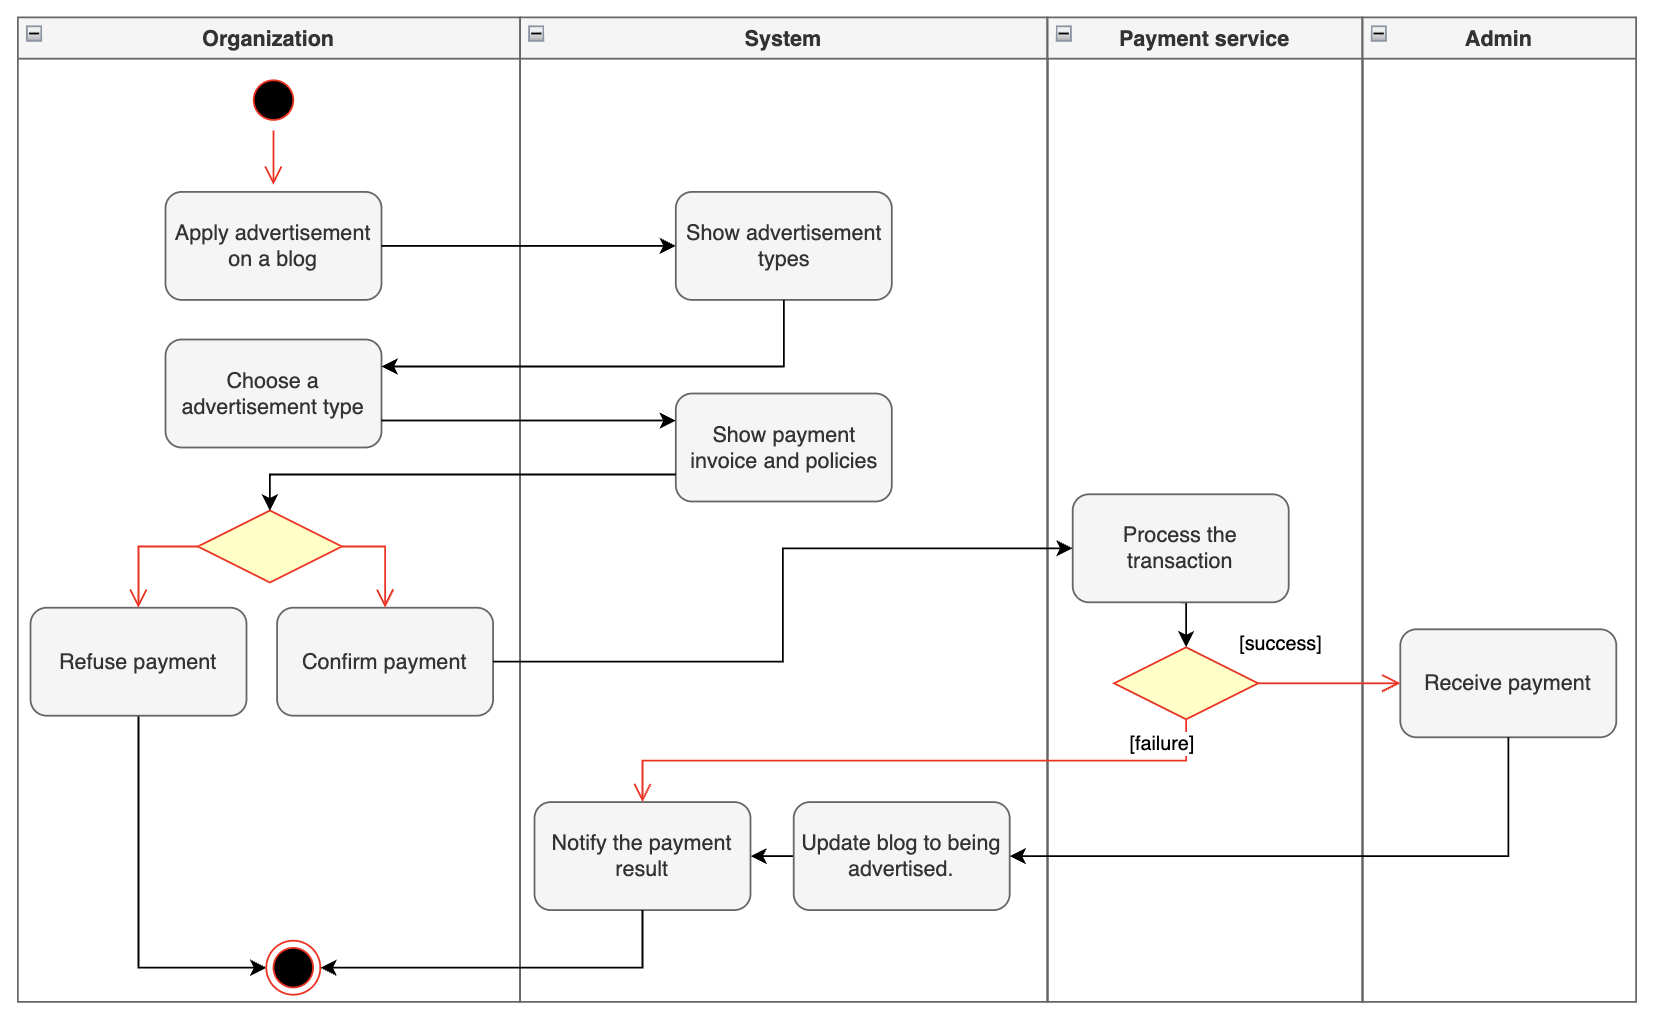
\includegraphics[width=0.7\textwidth]{Figures/payment.png}
\caption{Make payment activity diagram}
\label{fig:make-payment}
\end{figure}